\documentclass[a0,portrait]{a0poster}
\usepackage{multicol}
\usepackage{poster}
\usepackage{amsmath,amsthm,amssymb}
\usepackage{epstopdf}
\usepackage{xspace}
\usepackage{verbatim}
%\usepackage{sagetex}
\usepackage{circuitikz}
\usepackage{url}
\usepackage{cite}

%\usepackage{pst-all}
%\usepackage{pst-circ}

\usepackage{titlesec}
\titlespacing*{\subsubsection}{0pt}{*0}{*0}
\titlespacing*{\subsection}{0pt}{0pt}{*0}
\titlespacing*{\section}{0pt}{0pt}{*0}

\newcommand{\Bold}{\mathbf}
\setlength{\paperwidth}{34in}
\setlength{\paperheight}{45in}
\title{Homomorphic Cryptosystems}

\author{
Jeremy Caci, Ali Hajy, Jonah Jolley\\
Clark Rinker, Philip Robinson\\
Advisor : Dr. David Bover\\
Computer Science Department
}



\begin{document}
\maketitle

\def\fh{{\em Fully Homomorphic}\xspace}

\begin{multicols}{2}
\begin{slide}{Abstract}

We present a formal inquiry of the first fully homomorphic encryption scheme proposed by Craig Gentry in 2008. Moreover we introduce the first implementation of this cipher in the Python programming language. A fully homomorphic encryption scheme enables the execution of arbitrary operations on encrypted data without the decryption key which, put simply, allows for a third party to  store and manipulate sensitive information without the ability to interpret it. 

%The applications of an efficient fully homomorphic encryption system are potentially limitless. A contemporary example is cloud based email, where a decentralized server stores and serves encrypted user email. Furthermore, such a system would allow for users to request the server to perform search queries on stored data without loss of privacy. This is a particularly enticing scenario given the recent boom in portable devices and multiparty computation, both of which currently have serious security concerns. 

Our investigation includes a high level synopsis of the mathematics involved in fully homomorphic encryption, a complete demonstration of our implementation in Python, and finally a overview of the space and asymptotic time complexities of the proposed system. 


\end{slide}

\begin{slide}{Components}


\begin{multicols}{2}

\resizebox{\columnwidth}{!}{
\begin{circuitikz}\draw
(0,0) node[and port,scale=1.5] (myand) {}
(myand.in 1) node[anchor=east] {{\small \({b_0}\)}}
(myand.in 2) node[anchor=east] {{\small \({b_1}\)}}
(myand.out) node[anchor=west] {{\small\({b_0 \cdot b_1}\;(\text{mod }2)\)}}
;\end{circuitikz}
}
\begin{align*}
  c_i\cdot c_j &= \left(p\cdot q_i + 2\cdot n_i + b_i\right)\\&\;\cdot\left(p\cdot q_j + 2\cdot n_j + b_j\right)\\
  &= p\cdot\hat{q} + 2\cdot\hat{n} + \left(b_i\cdot b_j\right)
\end{align*}


\resizebox{\columnwidth}{!}{
\begin{circuitikz}\draw
(0,0) node[xor port,scale=1.5] (myand) {}
(myand.in 1) node[anchor=east] {{\small\({b_0}\)}}
(myand.in 2) node[anchor=east] {{\small\({b_1}\)}}
(myand.out) node[anchor=west] {{\small \({b_0 + b_1}\;(\text{mod } 2)\)}}
;\end{circuitikz}
}
\begin{align*}
  c_i+ c_j &= \left(p\cdot q_i + 2\cdot n_i + b_i\right)\\&\;+\left(p\cdot q_j + 2\cdot n_j + b_j\right)\\
%  &= p\cdot(q_i+q_j)+2\cdot(n_i+n_j) \\&\;+ b_i + b_j\\
  &= p\cdot\hat{q} + 2\cdot\hat{n} +\left(b_i+b_j\right)
\end{align*}




\end{multicols}

%\end{comment}

%Given a security parameter $\lambda$ we produce a $p \in \{0,1\}^{\lambda^2-1}|1$. Then for every bit $b_i$ we are encrypting we choose a random value $q_i \in \{0,1\}^{\lambda^5}$ as a means of distancing the data from the key. We then choose a random value $n_i \in \{0,1\}^{\lambda-1}|b_i$ which denotes noise. The cipher-bit $c_i = p\cdot q_i + n_i + b_i$. ($|x$ denotes that the value $x$ is concatinated onto the end of the bitstream.)

%Step 3 is only possible because we have chosen to force bit parity for cooresponding $n_k,b_k$ pairs. This forces the $\hat{n}+\hat{b}$ values together to be even. Eventhough they may seperately not be. 

%You have to trust this or do it by hand. (formal proofs not included)


\resizebox{\columnwidth}{!}{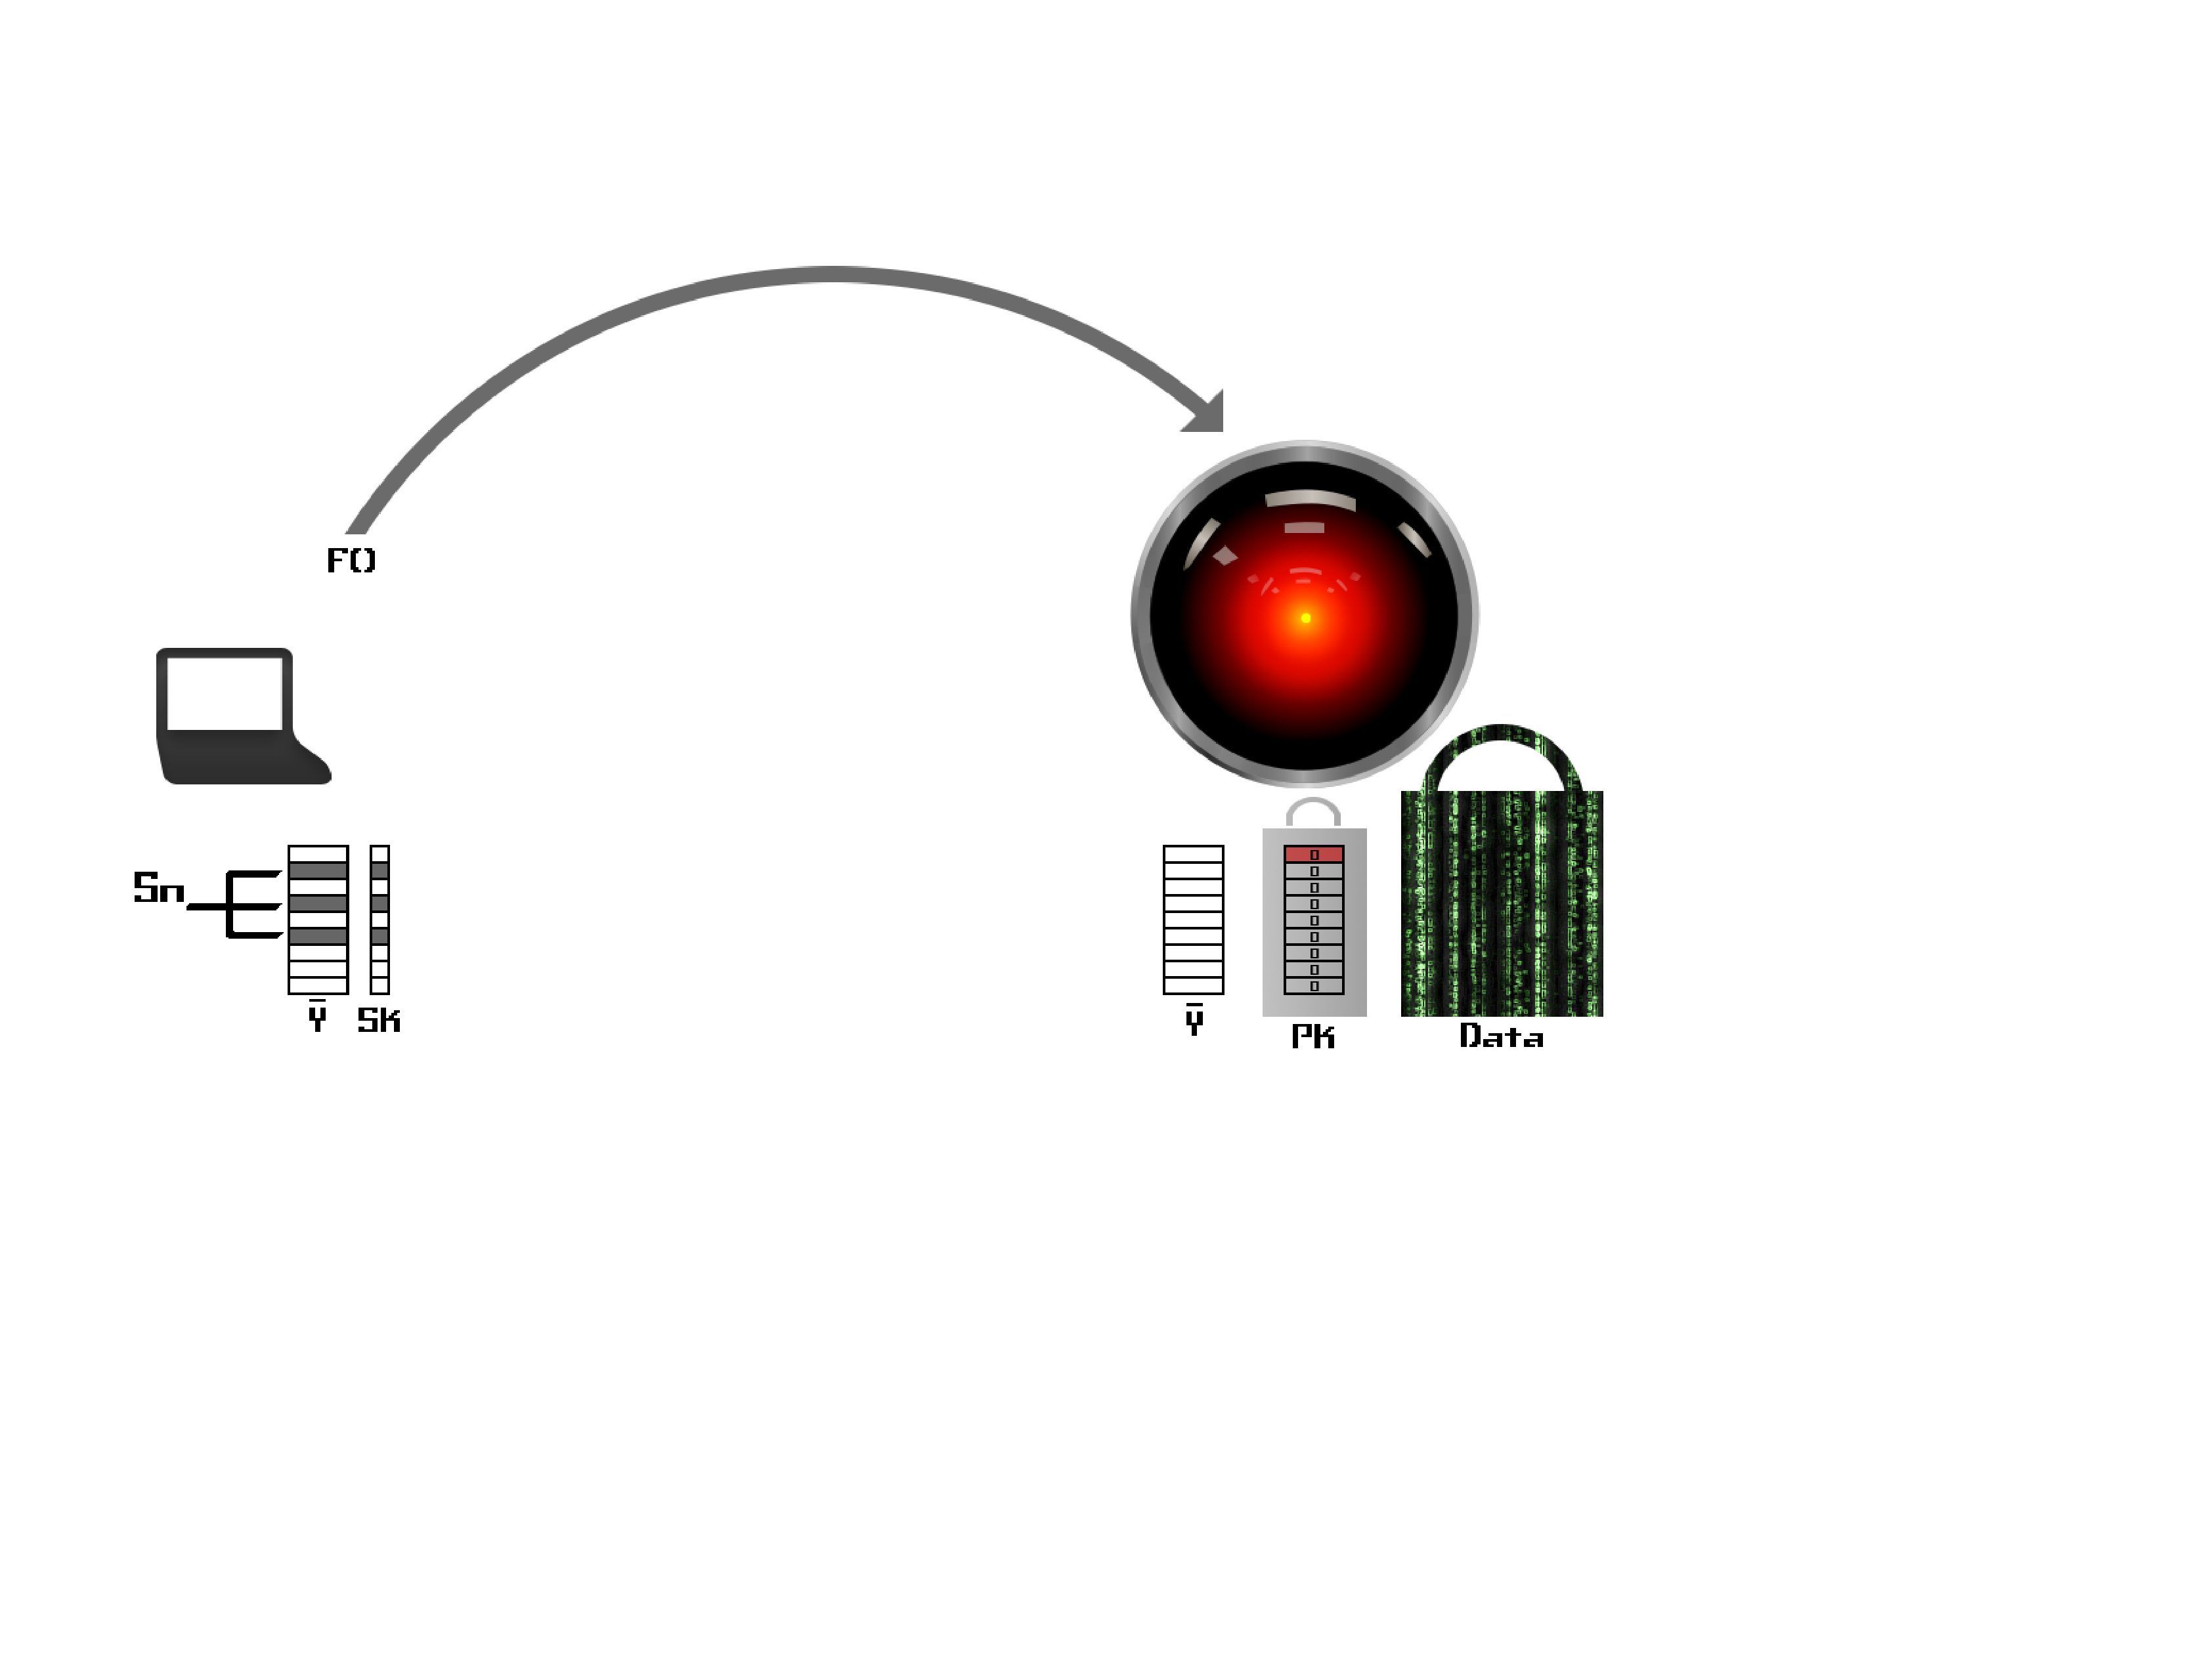
\includegraphics{infograph.eps}}


%An asymmetric encryption Scheme E has three algorithms:
%\section*{KeyGen}
%use lambda to generate two keys, a public encryption key pk that is available to everyone, and a secret decryption key sk.
%\section*{Encrypt}
%Will map a message to ciphertext using pk.
%\section*{Decrypt}
%will map the ciphertext back to the message using sk.
%Homomorphic Encryption scheme incorporates a fourth algorithm:
%\section*{Evaluate}
%Given pk, will perform operations over ciphertext to produce equivalent encrypted results%

Our implementation is comprised of five functions:


\subsection*{KeyGen}
\hspace{1em}Uses \(\lambda\) to generate two keys, a public key that is available to everyone, and a secret key that is only available to the client to be used in decryption. 

\subsection*{Encrypt}
\hspace{1em}Maps a plaintext message to a ciphertext using the public key.

\subsection*{Decrypt}
\hspace{1em}Maps a ciphertext back to its original message using the secret key.

\subsection*{Recrypt}
\hspace{1em}Encrypts a previously encrypted ciphertext using the public key, which effectively reduces the space and increases the integrity of the data. 

\subsection*{Evaluate}
\hspace{1em}Given the public key and a set of arbitrary operations, this function will execute each instruction over the entire ciphertext and return the encrypted results.


\end{slide}

\begin{slide}{Security}

Given a security parameter \(\lambda\) there exists a private key space of 

\[2^{(\lambda^2-2)} - (2^{\lambda^{2-1}})-1\]

The cryptographic hint uses the subset sum problem over a sparse subset. A brute force attack on this scheme requires the space 

\[\left(\begin{matrix}\beta = \lambda^5\\\alpha \end{matrix}\right)\approx \beta^\alpha\]

This shows that the security of this fully homomorphic encryption system is rival to that of most contemporary systems.

%The problem of cracking is {\em Soft NP-Complete}

%This is because as the security parameters grows, the searchspace and the cost of the operations grow. 
\end{slide}

\begin{slide}{Limitations}
\subsection*{Space Complexity}
  This cryptographic model has not yet been refined to a practical level. Encrypting data bitwise under these methods, such that the cipher text is cryptographically secure requires a great degree of noise/bloat to hide the pairity of our unencrypted message bidgit. 
\parskip 1em


 % \vspace{1em}
\resizebox{\columnwidth}{!}{
  \begin{tabular}{c|c|c|c|c|c}
     & {\small bit-size} &  {\small encrypted volume}  & \(\lambda = 8\) & \(\lambda = 16\) & \(\lambda = 64\) \\\hline 
    {\small bidgit} & 1 & \(\approx \lambda^7 \) & \(\approx\) 256 KB & 32 MB & 512 GB \\\hline
    {\small ``cadadr''} & 6 Bytes & & \(\approx\) 12 MB & 1.5 GB & 24 TB \\\hline
    {\small Declaration of Independence} & 8.5 KB & & \(\approx\) 17 GB & 2.1 TB & 34 PB\\
  \end{tabular}
  }%\end{center}
 % \vspace{1em}

%  What we also notice is that the storage space of encrypted data is linear \(\;\in\Theta(1)\) with respect to information size.  It is also important to note that operations can as much as double the space complexity over the addressed space, but this is often not over a large block of space.

\begin{comment}
\begin{align*}
f_{(1\text{ bit},64)}&=512\; GB\\
f_{(6\text{ Bytes},64)}&=(512\; GB)\cdot6\cdot 8\\&=24\; TB
\end{align*}
\end{comment}


\end{slide}





\begin{slide}{Next Steps}
  What we have accomplished is effective but not efficient. Although we recognize that this cryptographic system is not a practical one, we would like to make it as realistic as possible. Because we are dealing with voluminous data, we are planning to distribute the storage and operations load accross an entire lab using {\em Hadoop} distributed systems. 
%\parskip 1em 

  Because we are working with such large numbers, it is additionally very time-expensive to perform multiplication. The kids multiplication algorithm is \(\in\Theta(n^2)\), but even with Karatsuba's algorithm \(\approx\Theta(n\cdot\lg^* n)\) implemented in python we do not recieve sufficient speed up. We are planning to shuffle this task onto the video card of each machine using {\em PyCuda}, so that we can perform faster DFTs. By doing this we can gain speed in parallelization that we are normally unable to recieve with python derivatives.

  Finally, we are looking at shrinking our space complexity by migrating to supporting an n-ary system rather than a binary system. This means we'll need to more formally address definitions for our co-sets and ideals.% under \(\mathbb{Z}_{<+,\cdot>}\)
\end{slide}


\begin{slide}{Conclusion}
%Our Findings \\ Further Implementations \\ Python as a Vehicle

\subsection*{Our Implementation}
\hspace{1em}We were successful in being the first group to implement a fully homomorphic encryption system using the Python programming language. The concerns about the efficiency of Python were surmounted using alternative optimized computation libraries, namely PyPy. We addressed the time and space limitations of this encryption system by utilizing a distributed file system tool called {\em Hadoop} and a cluster of powerful computers available to us in Western's Computer Science Department. 

\subsection*{Feasibility} 
\hspace{1em}Even with the resources available to us, the overhead of this encryption scheme make a contemporary model impractical. The space required to encrypt and store a dataset with a sufficient security parameter is unreasonable. However, the concept of a fully homomorphic encryption scheme is still in its infancy, and since Craig Gentry's initial dissertation multiple papers have been published containing new and exciting optimizations to the original algorithm. This combined with the rate at which modern hardware is advancing might make the idea of a functional fully homomorphic system possible in the future. 

\end{slide}

\begin{comment}
\renewcommand{\refname}{}
\begin{slide}{Bibliography}
\nocite{*}
\bibliography{mybib}{}
\bibliographystyle{plain}
\end{slide}
\end{comment}
\end{multicols}

\end{document}
